\documentclass[11pt,a4paper,oneside]{report}
\usepackage[T1]{fontenc}
\usepackage[utf8]{inputenc}
\usepackage{mathpazo}

\usepackage{microtype}
\usepackage[margin=2.5cm,headheight=14pt]{geometry}
\usepackage{amsmath,amssymb,amsthm}
\usepackage{graphicx,booktabs,array,enumitem,xcolor}
\usepackage[most]{tcolorbox}
\usepackage{fancyhdr}
\usepackage{titlesec}
\usepackage[numbers,sort&compress]{natbib}
\usepackage[colorlinks=true,linkcolor=blue!50!black,citecolor=green!40!black,urlcolor=blue!60!black]{hyperref}
\usepackage[capitalise,noabbrev]{cleveref}
\usepackage{listings}

\definecolor{accent}{HTML}{4A2F7A}
\titleformat{\chapter}[display]{\normalfont\huge\bfseries\color{accent}}{\large\scshape Chapter \thechapter}{8pt}{\Huge}
\titlespacing*{\chapter}{0pt}{-10pt}{18pt}
\pagestyle{fancy}\fancyhf{}
\fancyhead[L]{\small\scshape\leftmark}\fancyhead[R]{\small H.~Tureli}
\fancyfoot[C]{\thepage}
\renewcommand{\headrulewidth}{0.3pt}
\setlist{itemsep=2pt,topsep=4pt}

\newtheorem{theorem}{Theorem}[chapter]
\newtheorem{proposition}[theorem]{Proposition}
\newtheorem{lemma}[theorem]{Lemma}
\theoremstyle{definition}
\newtheorem{definition}[theorem]{Definition}
\newtheorem{example}[theorem]{Example}
\theoremstyle{remark}
\newtheorem{remark}[theorem]{Remark}

\newtcolorbox{keybox}[1][]{colback=accent!4,colframe=accent!70,fonttitle=\bfseries,title={#1},sharp corners,boxrule=0.6pt}
\newtcolorbox{notebookbox}{colback=green!3,colframe=green!45!black,sharp corners,boxrule=0.5pt,
  title={\small\bfseries Python sheet},fonttitle=\small}
\newtcolorbox{correctionbox}{colback=orange!5,colframe=orange!70!black,sharp corners,boxrule=0.5pt,
  title={\small\bfseries A note on the original slides},fonttitle=\small}
\newtcolorbox{qabox}{colback=gray!4,colframe=gray!55,sharp corners,boxrule=0.5pt,breakable,
  title={\bfseries Questions and answers},fonttitle=\normalsize}
\newcommand{\Qu}[1]{\item[\textbf{Q.}] #1}
\newcommand{\A}[1]{\\[-2pt]\textbf{A.}~#1\par\smallskip}
\newenvironment{qa}{\begin{qabox}\begin{enumerate}[leftmargin=1.6em,label={}]}{\end{enumerate}\end{qabox}}

\lstset{basicstyle=\ttfamily\small,columns=fullflexible,keepspaces=true,frame=single,
  rulecolor=\color{gray!40},backgroundcolor=\color{gray!4},xleftmargin=4pt,xrightmargin=4pt,
  keywordstyle=\color{accent}\bfseries,language=Python,showstringspaces=false}

\newcommand{\Z}{\mathbb{Z}}\newcommand{\QQ}{\mathbb{Q}}
\newcommand{\sheet}[1]{\texttt{book/#1}}
\newcommand{\code}[1]{\texttt{#1}}

\hypersetup{pdftitle={Euler's Tonnetz, Graph Theory and Geometry: A Tutorial Review},pdfauthor={Hale Tureli}}

\begin{document}
\begin{titlepage}
\centering
\vspace*{2.2cm}
{\color{accent}\rule{\linewidth}{1pt}}\\[14pt]
{\Huge\bfseries Euler's Tonnetz, Graph Theory\\[6pt] and Geometry}\\[12pt]
{\LARGE A Tutorial Review with Reproducible Python Sheets}\\[10pt]
{\color{accent}\rule{\linewidth}{1pt}}\\[2cm]
{\Large Hale Tureli}\\[6pt]
{\large Technical Report}\\[4pt]
{\normalsize September 2026}\\[2.5cm]
\begin{minipage}{0.82\linewidth}\small
\textbf{Abstract.} The Tonnetz (``tone network'') of Euler arranges the twelve pitch classes so that consonant
triads become triangles of a lattice. Read as mathematics, it is simultaneously a graph, a group action and a
triangulated surface. This report is a self-contained tutorial that develops the subject from first principles
for students while collecting the computational and empirical literature for researchers. We (i) build the
Tonnetz as a quotient of $\Z^2$ and prove it is a torus; (ii) study the neo-Riemannian operations $P$, $L$, $R$
and the dual ``chicken-wire'' graph; (iii) enumerate its Hamiltonian cycles, confirming $124$ directed
($62$ undirected) cycles and classifying them into eight orbits under transposition and inversion;
(iv) reproduce Catanzaro's topological classification of generalized Tonnetze for $N=12$;
(v) analyse seventh-chord and edge-labelled Tonnetze, where non-orientable surfaces such as the real
projective plane appear; and (vi) place four public corpora (Bach, Beethoven, two pop collections) on the
Tonnetz, finding that classical progressions are more Tonnetz-compact than their own shuffled chords while pop
progressions are not. Every chapter ends with questions and answers, and every number is reproduced by an
executable notebook in the accompanying repository.
\end{minipage}
\vfill
{\small Developed from the DREAMS 2025 project presentation \emph{Euler's Tonnetz, Graph Theory, and Geometry}
by S.~Doran, K.~Tsang and H.~Tureli (advisor: J.~Jones).}
\end{titlepage}

\pagenumbering{roman}
\tableofcontents
\clearpage

\chapter*{How to read this report}
\addcontentsline{toc}{chapter}{How to read this report}
\markboth{How to read this report}{}
The report is written for two audiences at once. \emph{Students} (final-year school, first-year university, or
musicians curious about mathematics) should read Chapters~1--5 in order, running the matching Python sheet after
each chapter. \emph{Researchers} can skim Chapters~2--4 for notation and go straight to the computational results
in Chapters~5--8 and the open problems in Chapter~9.

\paragraph{Companion repository.} All code lives in a single repository with four parts:
\code{tonnetzkit/} (a small Python package), \code{book/} (ten Jupyter notebooks forming a Jupyter Book of ``Python
sheets''), \code{scripts/} (figure generation, data download and the corpus study), and \code{tests/} (regression
tests pinning every numerical claim in the text). Boxes like the one below point to the relevant sheet.
\begin{notebookbox}
\sheet{00\_welcome.ipynb} gives a five-minute tour: it builds the 24 triads, applies $P,L,R$, counts Hamiltonian
cycles and plays a chord progression, all with no external data.
\end{notebookbox}

\paragraph{Conventions.} Pitch classes are integers mod 12 with $C=0$, $C\sharp=1,\dots,B=11$. We write major
triads by their root (C, F$\sharp$) and minor triads with a lower-case ``m'' (Am). Sharps are used throughout, as in
the original slides; in 12-tone equal temperament A$\sharp$ and B$\flat$ name the same pitch class.

\paragraph{Relation to the original presentation.} The report expands every slide of the DREAMS 2025 presentation.
Where a slide simplified or mis-stated something, an orange box explains the correction; these are offered in the
spirit of peer review of our own work, not as criticism of a student presentation.

\clearpage
\pagenumbering{arabic}
\chapter{Introduction: a map of harmony}\label{ch:intro}

\section{Why a map?}
Musicians have always used spatial language for harmony: chords are ``close'' or ``distant'', a modulation
``travels'' to a ``remote'' key, a progression ``returns home''. The Tonnetz makes this language literal. It is a
diagram in which every point is a note and every small triangle is a chord, arranged so that geometric nearness
tracks a musical notion of nearness: two triangles that share an edge are two chords that share two notes and
can be connected by moving a single voice a short distance.

Once the picture is drawn, three branches of mathematics appear at once. As a \emph{graph} it invites questions
about paths and cycles: can we walk through all 24 major and minor chords, each exactly once, moving only between
neighbours? As a \emph{group action} it explains why transposing a progression preserves its shape. As a
\emph{surface} it has a topology: when the diagram is wrapped up so that each note appears only once, it becomes a
torus, and variants built from other chords become cylinders, spheres, M\"obius bands or even the real projective
plane. The goal of this report is to develop all three views carefully, to compute everything that can be
computed, and finally to test the map against real music.

\section{A short history}
\paragraph{Euler (1739).} Leonhard Euler's \emph{Tentamen novae theoriae musicae} \citep{euler1739} contains a
small lattice of note names in which horizontal neighbours differ by a perfect fifth and vertical neighbours by a
major third. For Euler, working in just intonation, the lattice was a way to organise frequency ratios built from
the primes 3 and 5; it was not yet a theory of chord progressions.

\paragraph{Nineteenth-century dualism.} Arthur von Oettingen \citep{oettingen1866} and Hugo Riemann
\citep{riemann1893} revived and extended the lattice (the German \emph{Tonnetz} is Riemann's usage). Their
harmonic ``dualism'' treated minor triads as mirror images of major ones, an idea that survives in the
inversional symmetry of Chapter~\ref{ch:prelims}.

\paragraph{Transformational and neo-Riemannian theory.} David Lewin's \emph{Generalized Musical Intervals and
Transformations} \citep{lewin1987} recast music theory in the language of groups acting on sets. Richard Cohn
then isolated three ``parsimonious'' transformations, $P$ (parallel), $L$ (leading-tone exchange) and $R$
(relative), that move a triad to another triad by shifting one voice by a semitone or a whole tone
\citep{cohn1996,cohn1997,cohn1998}. The Tonnetz became the natural stage for these operations, and a large body of
analysis of chromatic nineteenth-century music followed \citep{cohn2012}, extended later to popular music
\citep{capuzzo2004}.

\paragraph{Geometry and topology.} From the late 1990s mathematicians and theorists studied the Tonnetz as a
space. Douthett and Steinbach introduced the ``chicken-wire torus'', the dual graph on triads
\citep{douthett1998}; Crans, Fiore and Satyendra showed that the $PLR$ group is dihedral of order 24 and is the
dual of the transposition/inversion group \citep{crans2009}. Tymoczko connected chord spaces to orbifolds and
voice leading \citep{callender2008,tymoczko2011,tymoczko2012}, and Catanzaro classified the topology of every
``generalized Tonnetz'' built from a single trichord type in any equal temperament \citep{catanzaro2011}. Bigo and
collaborators represented chord collections as simplicial complexes and built the HexaChord software
\citep{bigo2013,bigo2016}. Yust \citep{yust2020}, Jevti\'c and \v{Z}ivaljevi\'c \citep{jevtic2021} and, most
recently, Boland and Hughston \citep{boland2025,boland2026} continue to generalise the construction, the latter
linking the Tonnetz to classical point--line configurations.

\paragraph{Computation and data.} In parallel, music information retrieval adopted the Tonnetz as a feature:
the tonal centroid of Harte, Sandler and Gasser \citep{harte2006} is implemented in the \code{librosa} library
\citep{mcfee2015} and used in chord recognition, and the Tonnetz has been used as an input representation for
neural networks \citep{chuan2018} and for genre classification from Tonnetz trajectories \citep{karystinaios2020}.
Large open chord corpora, notably ChoCo \citep{deberardinis2023} and Chordonomicon \citep{kantarelis2024}, now
make it possible to test Tonnetz-based hypotheses at scale; Xu, Hall and Rohrmeier's recent study of tonal
coherence on the Tonnetz across 2,800 pieces \citep{xu2026} is an example.

\section{What this report adds}
Beyond a unified tutorial exposition, the report contributes a set of verified, reproducible computations:
\begin{enumerate}
\item an independent enumeration of Hamiltonian cycles in the dual graph (62 undirected, 124 directed, as reported
by Albini and Antonini \citep{albini2009}) together with their classification into eight symmetry orbits and their
voice-leading costs (Chapter~\ref{ch:ham});
\item a machine-checked table of all twelve generalized Tonnetze in 12-tone equal temperament, including the
parity phenomenon that turns the chromatic strip into a M\"obius band for odd $N$ (Chapter~\ref{ch:topology});
\item a reconstruction of the presentation's whole-tone ``edge Tonnetz'' as a triangulated real projective plane,
contrasted with the actual pitch-class complex and with a Monte-Carlo census of edge-labelled gluings
(Chapter~\ref{ch:nonorient});
\item a four-corpus study with a shuffling null model (Chapter~\ref{ch:data}).
\end{enumerate}

\begin{keybox}[The one-sentence summary]
The Tonnetz is a triangulated torus whose vertices are the twelve notes and whose 24 triangles are the major
and minor triads; its dual is a 3-regular graph on those triads in which each edge is one of Cohn's
single-voice moves $P$, $L$ or $R$.
\end{keybox}

\begin{qa}
\Qu{In one sentence each, what are the three mathematical ``views'' of the Tonnetz used in this report?}
\A{As a graph (notes or chords joined by musical relations, studied through paths and cycles); as a group action
(transposition, inversion and the $P,L,R$ operations acting on chords); and as a surface (a triangulated torus
whose topology can be computed).}
\Qu{Why was Euler's original lattice not yet a torus?}
\A{Euler worked in just intonation, where no two lattice points have exactly the same frequency ratio, so the
lattice is an infinite plane. The torus appears only after identifying notes that are equal in 12-tone equal
temperament (Chapter~\ref{ch:tonnetz}).}
\Qu{Which three operations did Cohn call parsimonious, and what makes them parsimonious?}
\A{$P$, $L$ and $R$. Each keeps two notes of a triad fixed and moves the third by a semitone ($P$, $L$) or a
whole tone ($R$), so the voice leading is as small as possible between a major and a minor triad.}
\Qu{Name one audio-processing tool that uses the Tonnetz.}
\A{The tonal-centroid (``tonnetz'') feature of Harte, Sandler and Gasser, available as
\code{librosa.feature.tonnetz}; it projects a chroma vector onto three circles (fifths, minor thirds, major
thirds).}
\Qu{What is the practical difference between a tutorial review and a research article?}
\A{A tutorial review re-derives known results in a teachable order and points to the literature; this one also
adds reproducible code and a few new computations, but its main purpose is to make the field accessible.}
\end{qa}

\chapter{Mathematical preliminaries}\label{ch:prelims}
This chapter collects the small amount of algebra, graph theory and topology used later. Readers comfortable
with modular arithmetic, graphs and the Euler characteristic can skip to Chapter~\ref{ch:tonnetz}.

\section{Pitch classes and intervals}
In 12-tone equal temperament (12-TET) the octave is divided into twelve equal semitones. Two identifications
turn pitches into \emph{pitch classes}: \emph{octave equivalence} (C4 and C5 are the same class) and
\emph{enharmonic equivalence} (F$\sharp$ and G$\flat$ are the same key on the piano). The set of pitch classes is
then the cyclic group $\Z_{12}=\{0,1,\dots,11\}$ with addition mod 12, where $C=0$.

An \emph{interval} from $x$ to $y$ is $y-x \bmod 12$. The musically important ones here are the minor third (3),
major third (4) and perfect fifth (7). Note that $3+4=7$ and $3+4+5=12$: a stack of a minor third, a major third
and a perfect fourth (5) closes the octave. This numerical coincidence is the reason the Tonnetz exists.

\begin{definition}
A \emph{trichord} is a 3-element subset of $\Z_{12}$. The \emph{major triad} on root $r$ is $\{r,r+4,r+7\}$ and the
\emph{minor triad} on root $r$ is $\{r,r+3,r+7\}$.
\end{definition}

Going around the pitch-class circle, the three notes of a trichord cut it into three gaps $(n_1,n_2,n_3)$ with
$n_1+n_2+n_3=12$. The major triad has gaps $(4,3,5)$ and the minor triad $(3,4,5)$: the same numbers in the
opposite cyclic order. This \emph{interval partition} is the key parameter of Catanzaro's generalized Tonnetze
(Chapter~\ref{ch:topology}).

\section{Transposition, inversion and the dihedral group}
The \emph{transposition} $T_n(x)=x+n$ and the \emph{inversion} $I_n(x)=n-x$ are bijections of $\Z_{12}$. They
satisfy
\[
T_mT_n=T_{m+n},\qquad I_mI_n=T_{m-n},\qquad T_mI_n=I_{m+n},\qquad I_nT_m=I_{n-m}.
\]
The 24 maps $\{T_n,I_n\}$ form a group, the dihedral group $D_{12}$ of order 24 (the symmetries of a regular
12-gon: rotations are transpositions, reflections are inversions). $D_{12}$ acts on trichords; transposition
preserves major and minor, while every inversion swaps them: for example $I_0(\{0,4,7\})=\{0,8,5\}$, which is F
minor. Hence $D_{12}$ acts \emph{simply transitively} on the 24 consonant triads: for any two triads there is
exactly one $T_n$ or $I_n$ carrying one to the other.

\begin{remark}
Under the action of $D_{12}$ the 220 trichords of $\Z_{12}$ fall into 12 orbits (the trichordal \emph{set
classes}); under transpositions alone they fall into 19 orbits. \Cref{sec:gentonnetz} computes the topology of the
Tonnetz associated with each of the 12 set classes.
\end{remark}

\section{Graphs}
A \emph{graph} $G=(V,E)$ is a set of vertices with a set of edges, each joining two vertices. The \emph{degree}
of a vertex is its number of edges; a graph in which every vertex has degree 3 is \emph{cubic} (3-regular). A
graph is \emph{bipartite} if its vertices split into two parts with all edges running between the parts. The
\emph{distance} between two vertices is the number of edges on a shortest path, and the \emph{diameter} is the
largest distance.

\begin{definition}
A \emph{Hamiltonian cycle} in $G$ is a closed walk that visits every vertex exactly once and returns to its start.
A graph that has one is \emph{Hamiltonian}.
\end{definition}

Unlike its cousin the Eulerian circuit (traverse every \emph{edge} once, decided in linear time by checking vertex
degrees), deciding whether a graph is Hamiltonian is NP-complete in general. For the 24-vertex graphs of this
report, exhaustive backtracking is instantaneous (Chapter~\ref{ch:ham}).

If a graph is drawn on a surface without crossings, its \emph{dual} has one vertex per face and joins two faces
that share an edge. The dual of the triangulated Tonnetz is the graph of triads connected by $P$, $L$ and $R$.

\section{Simplicial complexes, Euler characteristic and surfaces}
\begin{definition}
An (abstract) \emph{simplicial complex} is a set $V$ of vertices together with a family of finite subsets
(simplices) closed under taking subsets. A 2-dimensional complex has vertices, edges (2-sets) and triangles
(3-sets). Its \emph{f-vector} is $(V,E,F)$ and its \emph{Euler characteristic} is $\chi=V-E+F$.
\end{definition}
A \emph{chord complex} has pitch classes as vertices and a chosen family of trichords as triangles
\citep{bigo2013}. A \emph{$\Delta$-complex} is the slightly more general object obtained by gluing triangles
along edges, where two triangles may share more than one edge; the Euler characteristic is defined the same way.

\paragraph{Homology in one paragraph.} Orient each edge and triangle. The boundary maps
$\partial_1$ (edge $\mapsto$ end $-$ start) and $\partial_2$ (triangle $\mapsto$ signed sum of its three edges)
are matrices; the \emph{Betti numbers} over a field $k$ are
\[
b_0=V-\operatorname{rk}\partial_1,\qquad b_1=E-\operatorname{rk}\partial_1-\operatorname{rk}\partial_2,\qquad
b_2=F-\operatorname{rk}\partial_2,
\]
and satisfy $\chi=b_0-b_1+b_2$. Informally $b_0$ counts components, $b_1$ independent loops and $b_2$ enclosed
cavities. Computing them over both $\QQ$ and $\Z_2$ detects non-orientability: a closed non-orientable surface
has $b_2=0$ over $\QQ$ but $b_2=1$ over $\Z_2$.

\begin{theorem}[Classification of closed surfaces]\label{thm:classification}
Every connected closed surface is homeomorphic to exactly one of: the sphere $S^2$, a connected sum of $g\ge1$ tori
(orientable, $\chi=2-2g$), or a connected sum of $k\ge1$ real projective planes (non-orientable, $\chi=2-k$).
It is determined by its Euler characteristic and its orientability.
\end{theorem}
This is exactly the theorem quoted on the presentation's slide ``Now how does the surface look?''. Orientable
surfaces always have \emph{even} $\chi$. Consequently a closed surface with $\chi=1$ must be non-orientable, with
$k=1$: it is the real projective plane $\mathbb{RP}^2$ (Chapter~\ref{ch:nonorient}). Surfaces with boundary
satisfy analogous rules: the cylinder (annulus) and the M\"obius band both have $\chi=0$ and are distinguished
by orientability.

\paragraph{Testing orientability by computer.} A triangulated surface is orientable if one can choose a cyclic
orientation for every triangle so that each shared edge is traversed in opposite directions by its two
triangles. A breadth-first search that propagates the orientation from triangle to triangle either succeeds or
finds a contradiction; this is \code{SimplicialComplex.is\_orientable()} in \code{tonnetzkit}.

\begin{notebookbox}
\sheet{01\_pitch\_classes.ipynb}: pitch-class arithmetic, the 24 permutations $\{T_n,I_n\}$ of the triads, and the
19 transposition classes and 12 set classes of trichords.
\end{notebookbox}

\begin{qa}
\Qu{Which two equivalences turn pitches into the 12 pitch classes?}
\A{Octave equivalence and enharmonic equivalence (the latter is exact only in equal temperament).}
\Qu{Verify that $I_0$ maps C major to F minor.}
\A{$I_0(x)=-x$: $\{0,4,7\}\mapsto\{0,8,5\}=\{F,A\flat,C\}$, the F minor triad.}
\Qu{Why does $D_{12}$ act simply transitively on the 24 consonant triads?}
\A{There are 24 group elements and 24 triads; transpositions move C major to every major triad, inversions move
it to every minor triad, and no nontrivial element fixes C major (its three gaps are all different, so it has no
symmetry). An orbit of size 24 with trivial stabiliser means simple transitivity.}
\Qu{What is the difference between a Hamiltonian cycle and an Eulerian circuit?}
\A{A Hamiltonian cycle visits every vertex once; an Eulerian circuit traverses every edge once. The latter exists
in a connected graph iff all degrees are even; the former has no such simple criterion.}
\Qu{A closed surface has $\chi=-2$. What can it be?}
\A{Either the orientable surface of genus 2 ($2-2g=-2$) or the non-orientable connected sum of four projective
planes ($2-k=-2$). Orientability decides which.}
\Qu{How can homology over two different fields reveal non-orientability?}
\A{For a closed connected surface, $b_2=1$ over $\Z_2$ always, but $b_2=1$ over $\QQ$ only if it is orientable.
A mismatch ($b_2=0$ over $\QQ$) therefore certifies non-orientability.}
\end{qa}

\chapter{The Tonnetz and why it is a torus}\label{ch:tonnetz}

\section{Construction as a lattice quotient}
Take the integer lattice $\Z^2$ and the group homomorphism
\[
\varphi:\Z^2\to\Z_{12},\qquad \varphi(i,j)=7i+4j \pmod{12}.
\]
Place lattice point $(i,j)$ in the plane at $i\,\mathbf e_1+j\,\mathbf e_2$ with $\mathbf e_1=(1,0)$ and
$\mathbf e_2=(\tfrac12,\tfrac{\sqrt3}{2})$, and label it with the note $\varphi(i,j)$. Then a step along
$\mathbf e_1$ adds a perfect fifth, a step along $\mathbf e_2$ adds a major third, and a step along
$\mathbf e_1-\mathbf e_2$ adds $7-4=3$, a minor third. Joining each point to its six neighbours triangulates the
plane (\cref{fig:lattice}); this is the layout of the TonnetzViz application \citep{cifka2016} used on the
original slides.

\begin{figure}[t]\centering
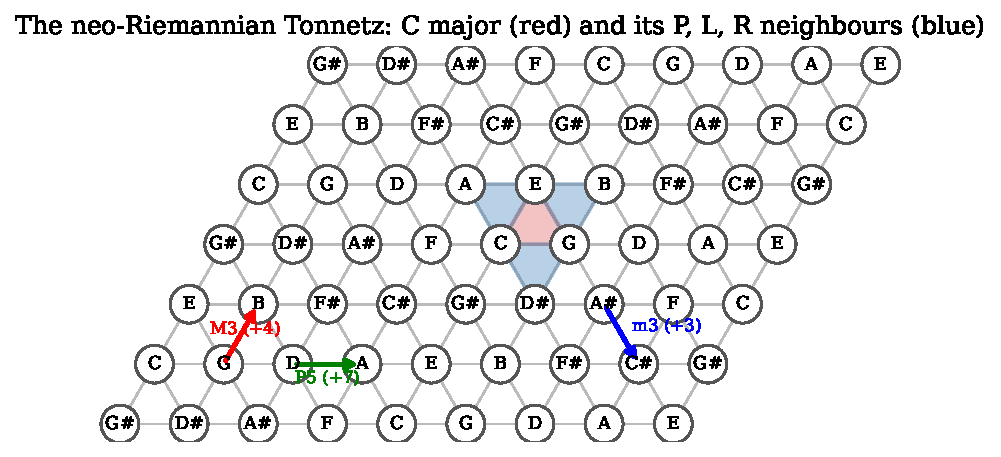
\includegraphics[width=0.86\linewidth]{figures/tonnetz_lattice.pdf}
\caption{The Tonnetz as a labelled triangular lattice. Upward triangles $\{x,x+4,x+7\}$ are major triads;
downward triangles are minor. C major (red) shares an edge with each of Cm, Em and Am (blue): these are its
$P$, $L$ and $R$ neighbours (Chapter~\ref{ch:plr}).}\label{fig:lattice}
\end{figure}

\begin{proposition}\label{prop:triangles}
The upward triangle with lower-left corner $x=\varphi(i,j)$ carries the notes $\{x,x+7,x+4\}$, the major triad on
$x$; the downward triangle on $(i{+}1,j),(i,j{+}1),(i{+}1,j{+}1)$ carries $\{x+7,x+4,x+11\}$, the minor triad on
$x+4$. Every major and minor triad occurs.
\end{proposition}
\begin{proof}
Direct substitution into $\varphi$. Since $\varphi$ is surjective (already $\varphi(i,0)=7i$ runs through all
residues because $\gcd(7,12)=1$), every root $x$ occurs, so every major and every minor triad occurs.
\end{proof}

\section{Identifying equal notes: the torus}
Each note appears infinitely often in the plane. To obtain one copy of each, identify lattice points with equal
labels, i.e.\ form the quotient $\Z^2/\ker\varphi$. The kernel is a sublattice of index 12, and one checks that
\[
\ker\varphi=\{(i,j):7i+4j\equiv0\}=\Z\,(4,-1)\oplus\Z\,(0,3).
\]
Musically, $(0,3)$ says that three major thirds make an octave ($C\to E\to G\sharp\to C$), and $(4,-1)$ that four
fifths up and a major third down return to the start ($C\to G\to D\to A\to E\to C$). The determinant of the basis
is $4\cdot3-(-1)\cdot0=12$, confirming the index.

\begin{theorem}\label{thm:torus}
The quotient of the triangulated plane by $\ker\varphi$ is a torus triangulated with $V=12$ vertices, $E=36$
edges and $F=24$ triangles; $\chi=0$. Its triangles are exactly the 24 major and minor triads.
\end{theorem}
\begin{proof}
A quotient of $\mathbb R^2$ by a rank-2 lattice of translations is a torus (glue opposite sides of the
fundamental parallelogram, \cref{fig:torus}). The lattice triangulation is invariant under the translations,
so it descends. Each vertex has six neighbours (at $\pm3,\pm4,\pm7$, which are six distinct residues), so
$E=12\cdot6/2=36$; each vertex lies in six triangles, so $F=12\cdot6/3=24$. By \cref{prop:triangles} the 24
triangles are the 24 triads, each once. Finally $12-36+24=0$.
\end{proof}

\begin{figure}[t]\centering
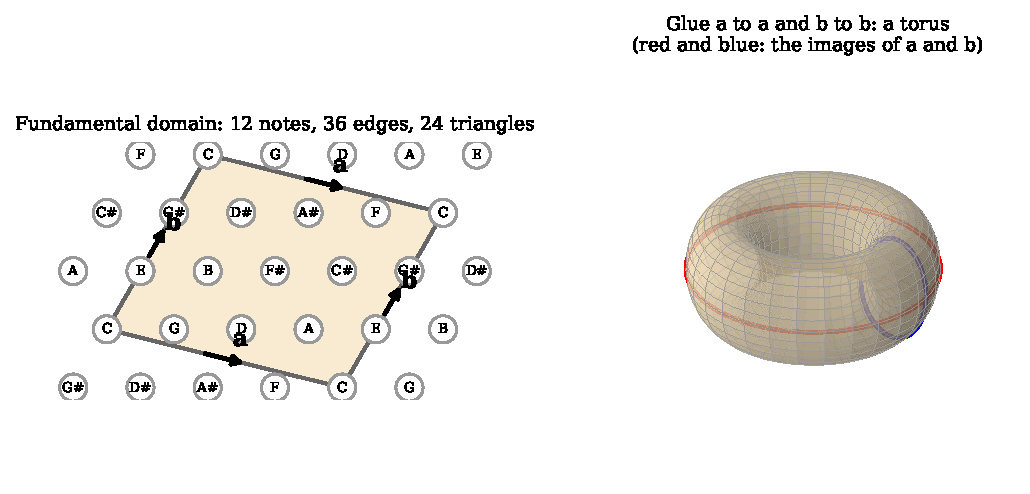
\includegraphics[width=0.92\linewidth]{figures/torus_domain.pdf}
\caption{Left: a fundamental domain spanned by $(4,-1)$ and $(0,3)$; all four corners are C. Gluing edge $a$
to $a$ and $b$ to $b$ (right) yields the torus.}\label{fig:torus}
\end{figure}

A computer check of \cref{thm:torus} is one line of \code{tonnetzkit}:
\begin{lstlisting}
K = generalized_tonnetz(3, 4, 5)   # all T/I images of {0, 3, 7}
K.summary()   # V=12, E=36, F=24, chi=0, betti (1,2,1), orientable -> torus
\end{lstlisting}
The Betti numbers $(1,2,1)$ are those of the torus: one component, two independent loops (the $a$- and
$b$-circles), one enclosed 2-cycle.

\begin{correctionbox}
The slide ``Hamiltonian cycles on a torus'' says the Tonnetz becomes a torus ``when you do octaves''. Octave
equivalence alone is not enough: in just intonation, as Harte, Sandler and Gasser point out, the Tonnetz is an
infinite plane even when octaves are ignored \citep{harte2006}. What closes the plane into a torus is
\emph{pitch-class} equivalence in 12-TET, which additionally equates enharmonic spellings. In particular three
pure major thirds ($5/4)^3=125/64$ fall short of an octave; only in equal temperament do they close exactly.
\end{correctionbox}

\section{Reading chords and progressions}
Because transposition $T_n$ acts on the lattice by translation, any chord or melody has a \emph{shape} on the
Tonnetz that is unchanged by transposition: all major triads are upward triangles and all minor triads downward.
Inversion $I_n$ acts by a point reflection, which is why it swaps the two triangle orientations. A progression
becomes a path of triangles; progressions whose consecutive chords share an edge move by one voice, and
progressions that ``jump'' across the diagram involve larger voice leading.

\paragraph{Other layouts.} Replacing $\varphi$ by $7i+3j$ (fifths and minor thirds) gives a mirror-image drawing of
the same complex, because the three generating intervals $\{3,4,5\}$ are unchanged. Genuinely different Tonnetze
arise only from different trichords (Chapter~\ref{ch:topology}) or from higher-dimensional lattices, for instance
Gollin's three-dimensional Tonnetz for seventh chords \citep{gollin1998}.

\begin{notebookbox}
\sheet{02\_tonnetz\_torus.ipynb}: print the lattice, find the kernel vectors by brute force, and verify
\cref{thm:torus}.
\end{notebookbox}

\begin{qa}
\Qu{Starting from C, which note is reached by the lattice step $(2,1)$?}
\A{$\varphi(2,1)=14+4=18\equiv6$, i.e.\ F$\sharp$: two fifths (C$\to$G$\to$D) and a major third (D$\to$F$\sharp$).}
\Qu{Explain in musical terms why $(0,3)\in\ker\varphi$.}
\A{Three consecutive major thirds, C--E--G$\sharp$--C, return to the starting pitch class (in 12-TET).}
\Qu{Why does each vertex of the Tonnetz have exactly six neighbours?}
\A{Its neighbours are at intervals $\pm3,\pm4,\pm7$, i.e.\ $3,9,4,8,7,5$: six distinct pitch classes.}
\Qu{Compute $\chi$ from the f-vector and name the surface.}
\A{$12-36+24=0$; the complex is orientable, so by \cref{thm:classification} it is the torus.}
\Qu{A student claims the Tonnetz is a sphere because ``it has no edges''. What is wrong?}
\A{Having no boundary does not determine the surface. Both the sphere and the torus are closed; the Euler
characteristic ($0$, not $2$) and the two independent loops ($b_1=2$) show it is a torus.}
\Qu{Why is every major triad an upward triangle?}
\A{Transposition acts by translation and preserves orientation; C major is upward, and every major triad is a
transposition of it.}
\end{qa}

\chapter{P, L, R and the dual graph}\label{ch:plr}

\section{Three parsimonious operations}
Two triangles of the Tonnetz share an edge exactly when the two triads share two notes. For each triad there are
three such neighbours, one across each edge, and they define three involutions on the set of 24 triads:
\begin{description}[leftmargin=1.2em]
\item[$P$ (parallel)] keeps the root and fifth and moves the third by a semitone: C $\leftrightarrow$ Cm.
\item[$L$ (leading-tone exchange)] keeps the third and fifth of a major triad and lowers the root a semitone:
C $\leftrightarrow$ Em (C--E--G $\to$ B--E--G).
\item[$R$ (relative)] keeps the root and third of a major triad and raises the fifth a whole tone:
C $\leftrightarrow$ Am (C--E--G $\to$ C--E--A).
\end{description}
In the lattice picture (\cref{fig:lattice}), $P$ flips a triangle across its fifth-edge, $L$ across its
minor-third edge and $R$ across its major-third edge. Each is its own inverse ($P^2=L^2=R^2=\mathrm{id}$) and each
swaps major and minor. Measured as total semitone motion of the voices, $P$ and $L$ cost 1 and $R$ costs 2; these
are the smallest possible voice leadings between a major and a minor triad, which is what Cohn means by
\emph{parsimonious} \citep{cohn1997}.

\section{The dual graph}
\begin{definition}
The \emph{$PLR$ graph} $\Gamma$ has the 24 consonant triads as vertices and an edge labelled $P$, $L$ or $R$ between
$t$ and $P(t)$, $L(t)$, $R(t)$.
\end{definition}
$\Gamma$ is the dual of the triangulated Tonnetz: vertices of $\Gamma$ are triangles of the Tonnetz and edges of $\Gamma$
cross edges of the Tonnetz. Drawn in the plane it is a hexagonal honeycomb (\cref{fig:dual}), and on the torus it
is Douthett and Steinbach's ``chicken-wire torus'' \citep{douthett1998}.

\begin{figure}[t]\centering
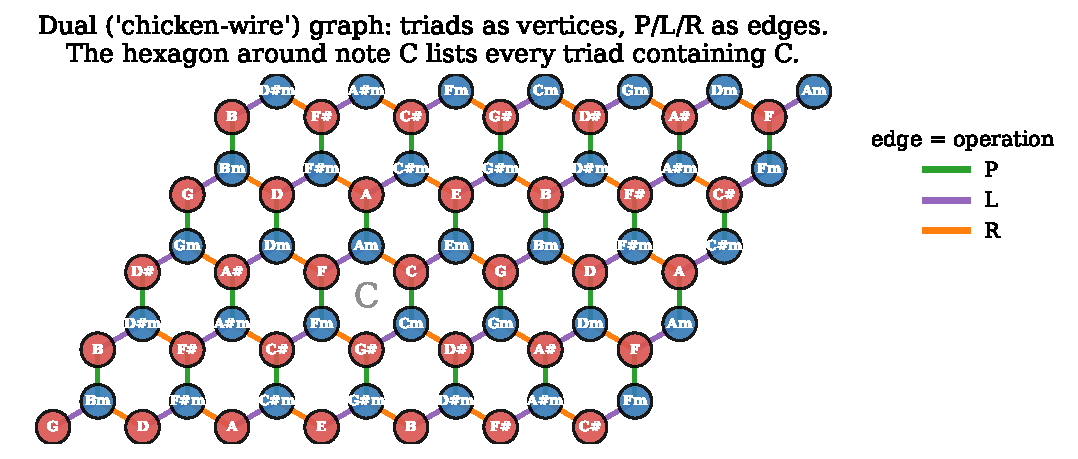
\includegraphics[width=0.9\linewidth]{figures/dual_graph.pdf}
\caption{A patch of the dual graph. Red vertices are major and blue are minor triads; edge colour gives the
operation. Every hexagonal face corresponds to one note of the Tonnetz and lists the six triads containing it.}
\label{fig:dual}
\end{figure}

\begin{proposition}\label{prop:gamma}
$\Gamma$ is connected, cubic, bipartite (majors versus minors) and has 24 vertices, 36 edges and diameter 5.
From any triad, the numbers of triads at distance $1,2,3,4,5$ are $3,6,8,5,1$.
\end{proposition}
\begin{proof}[Proof sketch]
Cubic and bipartite follow from the definitions ($P,L,R$ are distinct and each changes the mode). Edges:
$24\cdot3/2=36$. The distance profile is the same from every vertex because $D_{12}$ acts transitively and
commutes with $P,L,R$ (below); it is checked by breadth-first search in \sheet{03\_plr\_dual.ipynb}. The unique
triad at distance 5 from C major is B$\flat$ minor.
\end{proof}

\section{Faces and famous cycles}
Three families of short cycles in $\Gamma$ are central to neo-Riemannian analysis.

\paragraph{Hexagons: the triads around a note.} Alternately applying $P$, $L$, $R$ six times returns to the start.
From C, $(PLR)^2$ visits C, Cm, A$\flat$, Fm, F, Am: precisely the six triads that contain the note C. These
hexagons are the faces of $\Gamma$ on the torus; there are 12 of them, one per pitch class, and $\Gamma$ has
$V-E+F=24-36+12=0$, as a graph embedded in the torus must.

\paragraph{Hexatonic cycles.} $(PL)^3$ from C gives C, Cm, A$\flat$, A$\flat$m, E, Em: the six triads contained in
the hexatonic scale $\{0,3,4,7,8,11\}$. There are four such cycles, Cohn's \emph{hexatonic systems}
\citep{cohn1996}, central to his account of late-Romantic ``maximally smooth'' progressions.

\paragraph{Octatonic cycles.} $(PR)^4$ gives eight triads (C, Cm, E$\flat$, E$\flat$m, F$\sharp$, F$\sharp$m, A, Am) in an
octatonic scale; there are three such cycles.

\paragraph{The $LR$ chain.} $(LR)^{12}$ visits all 24 triads, alternating major and minor while the major roots
descend (or ascend) by fifths: C, Em, G, Bm, D, $\dots$ Long stretches of this chain occur in the repertoire; a
celebrated example is a passage in the scherzo of Beethoven's Ninth Symphony discussed by Cohn \citep{cohn1997}.
We meet this cycle again as the most symmetric Hamiltonian cycle in Chapter~\ref{ch:ham}.

\begin{correctionbox}
The slide ``Hamiltonian cycles (again)'' states that ``going around a hexagon'' gives
C $\to$ Am $\to$ F $\to$ Dm $\to$ G $\to$ Em $\to$ C. Checking each step against $\Gamma$ shows that five steps are
edges ($R,L,R$ and then $R,L$) but Dm $\to$ G is not: D--F--A and G--B--D share only one note (PLR distance 3).
The progression is a diatonic chain of falling thirds, not a face of the dual graph. The hexagon through C and Am
is C--Cm--A$\flat$--Fm--F--Am (the triads containing C), or, around the note E, C--Em--E--C$\sharp$m--A--Am.
\end{correctionbox}

\section{The $PLR$ group and its dual}
Let $\mathcal{G}=\langle P,L,R\rangle$ be the group of permutations of the 24 triads generated by the three
involutions. A direct computation (\sheet{03\_plr\_dual.ipynb}) shows $|\mathcal G|=24$; in fact $\mathcal G$ is
already generated by $L$ and $R$, since $RL$ has order 12, and $\mathcal G\cong D_{12}$. The deeper structural
fact is:

\begin{theorem}[Crans--Fiore--Satyendra \citep{crans2009}]
The $PLR$ group and the $T/I$ group are both dihedral of order 24, each acts simply transitively on the
consonant triads, and each is the centraliser of the other in the symmetric group on the 24 triads.
\end{theorem}
Informally: $P$, $L$ and $R$ are defined by \emph{internal} features of a chord (``keep root and fifth'') rather
than by absolute pitch, so they commute with transposition and inversion. For example
$P(T_5\,t)=T_5\,P(t)$ for every triad $t$; the notebook verifies this for all 24 triads. Transformational theorists
call this relationship \emph{duality} (Lewin's ``simply transitive group action'' \citep{lewin1987}); it explains
why a neo-Riemannian analysis can be transposed freely.

\section{Two metrics on triads}
Distances in $\Gamma$ count single-voice moves; the \emph{voice-leading distance} instead minimises the total
number of semitones moved, over all ways of pairing the notes. They agree on edges only up to the factor that
$R$ costs 2, and diverge more for larger moves: C $\to$ G (a fifth up) is two steps in $\Gamma$ ($L$ then $R$) with
voice-leading cost 3, while F $\to$ G (a whole step, as in IV $\to$ V) is four steps in $\Gamma$ with voice-leading
cost 6. This difference matters for the corpus study of Chapter~\ref{ch:data}.

\begin{notebookbox}
\sheet{03\_plr\_dual.ipynb}: build $\Gamma$, verify \cref{prop:gamma}, list the hexagonal, hexatonic and octatonic
cycles, test the slide's progression edge by edge, and generate $\langle P,L,R\rangle$.
\end{notebookbox}

\begin{qa}
\Qu{Compute $P$, $L$ and $R$ of A minor.}
\A{$P(\text{Am})=\text{A}$ (C$\to$C$\sharp$), $L(\text{Am})=\text{F}$ (E$\to$F), $R(\text{Am})=\text{C}$
(A$\to$G).}
\Qu{Why is $\Gamma$ bipartite?}
\A{Each of $P$, $L$, $R$ changes the mode, so every edge joins a major triad to a minor triad.}
\Qu{How many hexagonal faces does $\Gamma$ have on the torus, and why?}
\A{Twelve: each face is the set of triads containing a fixed note, and there are 12 notes. Check:
$\chi=24-36+12=0$.}
\Qu{Which triads lie on the hexatonic cycle through D major?}
\A{$(PL)^3$ from D: D, Dm, B$\flat$, B$\flat$m, F$\sharp$, F$\sharp$m.}
\Qu{Why do $P,L,R$ commute with transposition?}
\A{They are defined relative to a chord's own root, third and fifth, and transposition moves all three together;
so transposing first and then applying $P$ gives the same result as applying $P$ then transposing.}
\Qu{Give a progression that is short in voice-leading terms but long in $\Gamma$.}
\A{F $\to$ G: every voice moves a whole step (cost 6, small as a gesture and idiomatic as IV--V) but it takes four
$P/L/R$ steps, e.g.\ F$\xrightarrow{R}$Dm$\xrightarrow{L}$B$\flat\xrightarrow{R}$Gm$\xrightarrow{P}$G.}
\end{qa}

\chapter{Hamiltonian cycles through all 24 triads}\label{ch:ham}

\section{The question}
Is there a chord progression that visits each of the 24 major and minor triads exactly once, moving only by
$P$, $L$ or $R$, and returns to where it started? In graph language: is $\Gamma$ Hamiltonian, and if so, how
many Hamiltonian cycles does it have? The question was posed and answered by Albini and Antonini
\citep{albini2009}, who enumerated and classified the cycles and discussed their compositional use; Albini and
Bernardi later developed Hamiltonian graphs as harmonic tools more broadly \citep{albini2017}. The presentation
slide asks the natural follow-up: \emph{do they sound better?}

Two counting conventions must be fixed first. A cycle can be traversed in two directions and started at any of
its 24 vertices. We call a \emph{directed} cycle a cyclic sequence with a chosen direction, and an
\emph{undirected} cycle the underlying set of 24 edges. Each undirected cycle corresponds to exactly two directed
ones.

\section{Enumeration by backtracking}
Because every vertex of $\Gamma$ has degree 3, a depth-first search that extends a path one vertex at a time and
backtracks on dead ends explores at most $2^{23}$ branches; in practice far fewer survive. The implementation in
\code{tonnetzkit.graphs} is:
\begin{lstlisting}
def hamiltonian_cycles(G, start):
    path, seen, out = [start], {start}, []
    def rec(v):
        if len(path) == len(G):
            if G.has_edge(v, start) and path[1] < path[-1]:  # keep one direction
                out.append(list(path))
            return
        for w in G.neighbors(v):
            if w not in seen:
                seen.add(w); path.append(w); rec(w); path.pop(); seen.discard(w)
    rec(start); return out
\end{lstlisting}
Fixing the start vertex removes the 24-fold rotational redundancy; the comparison \code{path[1] < path[-1]}
keeps one of the two directions. On a laptop the search finishes in about 0.1 seconds.

\begin{proposition}\label{prop:hamcount}
$\Gamma$ has exactly $62$ undirected Hamiltonian cycles, i.e.\ $124$ directed Hamiltonian cycles. Starting from a
fixed triad there are $470$ directed Hamiltonian \emph{paths}, of which $124$ end at a neighbour of the start and
close into cycles.
\end{proposition}
The count 124 agrees with Albini and Antonini \citep{albini2009}, and the slide's ``62 such cycles up to
ordering'' is the undirected count. Both are pinned by the regression test \code{test\_hamiltonian\_counts}.

\section{Classification up to symmetry}
Since $T_n$ and $I_n$ commute with $P,L,R$ they map Hamiltonian cycles to Hamiltonian cycles, so the 62 cycles
fall into orbits under $D_{12}$. Each orbit has size $24/|\mathrm{Stab}|$, where the stabiliser is the subgroup of
symmetries mapping the cycle to itself. Independently, one can read the sequence of edge labels around each
cycle, a cyclic word of length 24 in the letters $P,L,R$, and consider it up to rotation and reversal. Because
symmetries preserve labels, cycles in the same orbit have the same word; our computation shows the converse also
holds here.

\begin{table}[t]\centering\footnotesize\setlength{\tabcolsep}{4pt}
\begin{tabular}{@{}cccccl@{}}\toprule
Orbit & \#$P$ & \#$L$ & \#$R$ & VL (semitones) & Cyclic word (up to rotation/reversal)\\\midrule
1  & 0  & 12 & 12 & 36 & $(LR)^{12}$\\
2  & 6  & 6  & 12 & 36 & $(LRPR)^6$\\
3  & 8  & 12 & 4  & 28 & $(LPLPLR)^4$\\
4  & 9  & 3  & 12 & 36 & $(LRPRPRPR)^3$\\
4  & 6  & 6  & 12 & 36 & $(LRLRPRPR)^3$\\
12 & 11 & 9  & 4  & 28 & \texttt{LPLPLRPLPLPRPLPLPRPLPLPR}\\
12 & 7  & 9  & 8  & 32 & \texttt{LPLRLPRLRPRLRPLRLPLRPLPR}\\
24 & 7  & 9  & 8  & 32 & \texttt{LPLRLPRLRLPLRPLPRPLRPRLR}\\\midrule
\multicolumn{6}{@{}l}{Total: $1+2+3+4+4+12+12+24=62$ undirected cycles in 8 orbits.}\\\bottomrule
\end{tabular}
\caption{The eight classes of Hamiltonian cycles of $\Gamma$. Voice-leading cost counts 1 semitone for each $P$
and $L$ and 2 for each $R$.}\label{tab:ham}
\end{table}

\begin{figure}[t]\centering
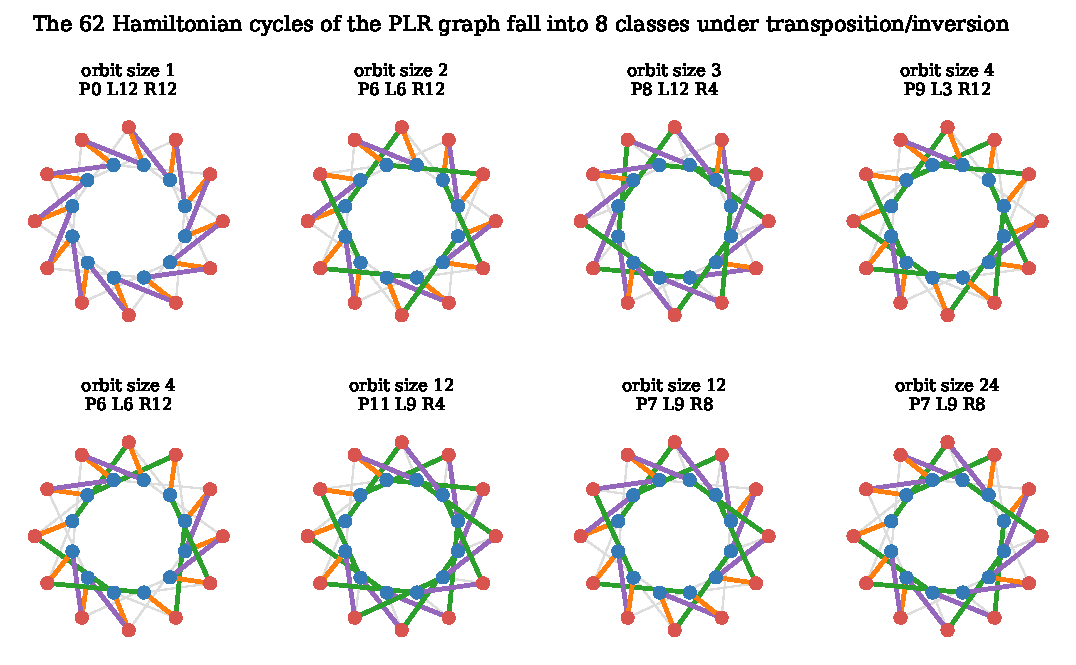
\includegraphics[width=\linewidth]{figures/hamiltonian_classes.pdf}
\caption{One representative of each class. Majors (red) lie on the outer ring ordered by fifths, each relative
minor (blue) just inside. Edge colours: $P$ green, $L$ purple, $R$ orange.}\label{fig:hamclasses}
\end{figure}

\Cref{tab:ham} and \cref{fig:hamclasses} summarise the result. Several observations are worth drawing out.
\begin{enumerate}
\item The $(LR)^{12}$ cycle is the unique cycle fixed by every symmetry. It is the ``circle of fifths with
relatives'': C, Em, G, Bm, D, F$\sharp$m, $\dots$
\item Every cycle uses $R$ at least four times and at most twelve. Because $R$ is the only operation that moves a
voice by a whole tone, the total voice leading ranges from 28 to 36 semitones: the classes of orbit size 3 and 12
with only four $R$ moves are the \emph{smoothest} complete tours of the triads.
\item Two pairs of classes share the same letter counts (6/6/12 and 7/9/8) but differ in word order, so the
letter counts alone do not classify cycles.
\end{enumerate}

\section{Do they sound better?}
The presentation asks whether Hamiltonian cycles sound better than other progressions. The mathematics cannot
answer this, and to our knowledge no controlled perceptual study has addressed it. What can be said is
structural: a Hamiltonian cycle uses maximal harmonic variety (every triad once) with minimal voice leading at every
step, a combination composers have exploited deliberately: Cannas and Andreatta point to pieces by Giovanni Albini and
Moreno Andreatta built on such cycles \citep{cannas2018}. A proper test would compare listener ratings of Hamiltonian cycles
against controls such as random walks on $\Gamma$ (same step size, but with repeats) and random orderings of the
24 triads (same variety, larger steps), matched for tempo, register and voicing. \Cref{ch:outlook} returns to this
as an open project, and \sheet{09\_research\_sandbox.ipynb} generates candidate stimuli.

\begin{notebookbox}
\sheet{04\_hamiltonian.ipynb}: enumerate the cycles, reproduce \cref{tab:ham}, and \emph{listen} to the smoothest
cycle and to the $(LR)^{12}$ cycle, synthesised in the notebook.
\end{notebookbox}

\begin{qa}
\Qu{Reconcile the numbers 62 and 124.}
\A{124 counts directed cycles (a direction of travel is chosen); each undirected cycle gives two directed ones, so
there are 62 undirected cycles.}
\Qu{Why does fixing the start vertex not lose any cycles?}
\A{Every Hamiltonian cycle passes through every vertex, in particular through the chosen start.}
\Qu{What is the orbit size of a cycle whose stabiliser has order 8?}
\A{$24/8=3$ (orbit--stabiliser theorem). This is the third row of \cref{tab:ham}.}
\Qu{Explain why the $(LR)^{12}$ cycle is unique among cycles using only $L$ and $R$.}
\A{$L$ and $R$ are involutions, so a walk using only them must alternate (repeating a letter would return to the
previous triad). The two alternating walks from a given triad are the same cycle in opposite directions, and it
closes only after 24 steps because $RL$ has order 12 on major triads.}
\Qu{Which Hamiltonian cycles minimise total voice leading, and what is the minimum?}
\A{Those with exactly four $R$ moves, the classes of orbit size 3 and 12 (first of the two 12s) in \cref{tab:ham},
with 28 semitones.}
\Qu{Design a control condition for the question ``do Hamiltonian cycles sound better?''.}
\A{For example, random walks of 24 steps on $\Gamma$ (same local smoothness, repeated chords allowed) and random
permutations of all 24 triads (same variety, larger steps), rendered identically and rated blind.}
\end{qa}

\chapter{Generalized Tonnetze and their topology}\label{ch:topology}

\section{From one trichord to a whole space}\label{sec:gentonnetz}
The classical Tonnetz is built from a single chord type: all transpositions and inversions of $\{0,4,7\}$. Nothing
prevents us from starting with any other trichord. Following Catanzaro \citep{catanzaro2011}, fix an equal
temperament $\Z_N$ and a partition $N=n_1+n_2+n_3$ into positive parts, and let
\[
\mathcal C(n_1,n_2,n_3)=\text{the chord complex whose triangles are all } T_t\text{ and } I_t\text{ images of }
\{0,\;n_1,\;n_1+n_2\}.
\]
Its vertices are the notes that occur, its edges are the note pairs that occur inside some chord, and its triangles
are the chords. The classical Tonnetz is $\mathcal C(3,4,5)$ in $\Z_{12}$. Related constructions include Cohn's
parsimonious trichords \citep{cohn1997}, Tymoczko's generalized Tonnetz of voice-leading lattices
\citep{tymoczko2012}, Bigo et al.'s chord-based complexes \citep{bigo2013}, and Yust's Tonnetze and ``Zeitnetze''
\citep{yust2020}; Jevti\'c and \v{Z}ivaljevi\'c prove that sufficiently generic higher-dimensional analogues
triangulate tori $T^{k-1}$ \citep{jevtic2021}.

Catanzaro's theorem \citep{catanzaro2011} classifies all these spaces for every $N$: the torus is the most common
outcome, especially as $N$ grows; the other possibilities are single 2-simplices, boundaries of tetrahedra, the
``harmonic strip'' (a cylinder or M\"obius band), and, for trichords containing a tritone, a ``circle of
tetrahedra boundaries'' related to Peck's Klein-bottle Tonnetz.

\section{All twelve cases for $N=12$, computed}
Up to transposition and inversion there are twelve trichord types in 12-TET. \Cref{tab:gentonnetz} lists the
complex of each, computed with \code{generalized\_tonnetz} and classified by the procedure of
Chapter~\ref{ch:prelims}: count components, check that every edge lies in at most two triangles, compute $\chi$
and orientability, then apply \cref{thm:classification}.

\begin{table}[t]\centering\small
\begin{tabular}{@{}llccccl@{}}\toprule
$(n_1,n_2,n_3)$ & Example chord & $V$ & $E$ & $F$ & $\chi$ & Space (Betti numbers over $\QQ$)\\\midrule
(1,1,10) & C--C$\sharp$--D cluster & 12 & 24 & 12 & 0 & cylinder (harmonic strip); (1,1,0)\\
(1,2,9)  & C--C$\sharp$--D$\sharp$ & 12 & 36 & 24 & 0 & torus; (1,2,1)\\
(1,3,8)  & C--C$\sharp$--E & 12 & 36 & 24 & 0 & torus; (1,2,1)\\
(1,4,7)  & C--C$\sharp$--F & 12 & 36 & 24 & 0 & torus; (1,2,1)\\
(1,5,6)  & C--C$\sharp$--F$\sharp$ & 12 & 30 & 24 & 6 & not a surface (edges in 4 triangles); (1,1,6)\\
(2,2,8)  & C--D--E & 12 & 24 & 12 & 0 & two cylinders (one per whole-tone scale); (2,2,0)\\
(2,3,7)  & C--D--F & 12 & 36 & 24 & 0 & torus; (1,2,1)\\
(2,4,6)  & C--D--F$\sharp$ & 12 & 30 & 24 & 6 & two components, not surfaces; (2,2,6)\\
(2,5,5)  & C--D--G & 12 & 24 & 12 & 0 & cylinder; (1,1,0)\\
(3,3,6)  & diminished C--E$\flat$--G$\flat$ & 12 & 18 & 12 & 6 & three tetrahedron boundaries (spheres); (3,0,3)\\
(3,4,5)  & major/minor triads & 12 & 36 & 24 & 0 & \textbf{torus}; (1,2,1)\\
(4,4,4)  & augmented C--E--G$\sharp$ & 12 & 12 & 4 & 4 & four disjoint triangles; (4,0,0)\\\bottomrule
\end{tabular}
\caption{Generalized Tonnetze in 12-TET. Betti numbers over $\Z_2$ coincide with those over $\QQ$ in every row.
Reproduced in \sheet{05\_generalized\_tonnetze.ipynb}; consistent with Catanzaro's classification.}
\label{tab:gentonnetz}
\end{table}

The table rewards careful reading.
\begin{itemize}
\item \emph{Six of the twelve types give tori}, including the classical Tonnetz. For a torus, each vertex must have
six distinct neighbours ($\pm n_1,\pm n_2,\pm n_3$ distinct), giving $E=36$ and $F=24$.
\item \emph{Symmetric chords collapse the space.} The augmented triad is fixed by $T_4$, so only four exist and
they are disjoint. The diminished triad lives inside a diminished-seventh collection of four notes whose four
3-subsets form the boundary of a tetrahedron, a sphere with $\chi=2$; three such collections give $\chi=6$.
\item \emph{Repeated gaps give strips.} When two gaps are equal (and no gap is a tritone or a third of the octave), the chord's neighbours coincide in pairs and the
complex is a long strip closing up on itself: a cylinder for $N=12$.
\item \emph{Tritones break the surface.} If a gap is 6, the tritone edge $\{x,x+6\}$ equals $\{x+6,x+12\}$ and is
shared by four triangles, so no neighbourhood looks like a disc. These are Catanzaro's circles of tetrahedra
boundaries.
\end{itemize}

\section{A parity phenomenon: cylinder or M\"obius band}
The chromatic cluster $\mathcal C(1,1,N-2)$ is a strip of triangles $\{x,x+1,x+2\}$ with the twisted edges of
consecutive triangles glued. Whether the strip closes with or without a half-twist depends on the parity of $N$.
Computing orientability for $5\le N\le15$ gives
\[
\mathcal C(1,1,N-2)\cong\begin{cases}\text{cylinder}, & N\text{ even},\\ \text{M\"obius band}, & N\text{ odd}.\end{cases}
\]
This is Catanzaro's harmonic strip ``in both its cylinder and M\"obius band variants''. The M\"obius case is the
first non-orientable space in this report; Chapter~\ref{ch:nonorient} meets closed non-orientable surfaces.

\paragraph{Beyond 12-TET.} In 19-tone equal temperament, looping over all 51 transposition classes of trichords
with \code{generalized\_tonnetz(a,b,c,n=19)} gives 42 tori and 9 M\"obius bands: since 19 is prime and odd, no chord
has transpositional symmetry and all harmonic strips twist. This illustrates the ``torus is generic'' part of
Catanzaro's theorem.

\begin{remark}[Why compute homology at all?]
Euler characteristic and orientability suffice for closed surfaces, but many musical complexes are not surfaces.
Betti numbers still describe them: $\mathcal C(1,5,6)$ has $b_2=6$ over $\QQ$, six independent enclosed
2-cycles, one per tritone pair. Topological signatures of this kind underlie the ``compliance'' measure of Bigo
et al.\ \citep{bigo2013} and persistent-homology fingerprints of musical pieces \citep{bergomi2016}.
\end{remark}

\begin{notebookbox}
\sheet{05\_generalized\_tonnetze.ipynb}: regenerate \cref{tab:gentonnetz} as a data frame, watch the harmonic strip
twist for odd $N$, and extend the table to 19-TET.
\end{notebookbox}

\begin{qa}
\Qu{How many trichord types are there in 12-TET up to transposition only, and up to transposition and inversion?}
\A{19 and 12. Inversion identifies a type with its mirror image, e.g.\ major (4,3,5) with minor (3,4,5).}
\Qu{Why does $\mathcal C(4,4,4)$ have only four triangles?}
\A{The augmented triad is invariant under $T_4$ and under inversion, so its $24$ images coincide in groups of six:
$24/6=4$ distinct triads, pairwise disjoint.}
\Qu{Show that each component of $\mathcal C(3,3,6)$ is a sphere.}
\A{A component is a diminished-seventh collection $\{x,x+3,x+6,x+9\}$; every 3-subset is a diminished triad, so
the four triangles form a tetrahedron boundary: $V-E+F=4-6+4=2$.}
\Qu{Why is $\mathcal C(1,5,6)$ not a surface?}
\A{Its tritone edges each lie in four triangles; around such an edge the space looks like four half-planes meeting
along a line, not like a plane.}
\Qu{For which $N$ is the chromatic strip a M\"obius band?}
\A{For odd $N$; for even $N$ it is a cylinder.}
\Qu{Name two spaces in \cref{tab:gentonnetz} with the same Euler characteristic but different topology.}
\A{The torus and the cylinder both have $\chi=0$; the torus is closed with $b_1=2$, the cylinder has boundary and
$b_1=1$. Euler characteristic alone does not classify spaces with boundary or with several components.}
\end{qa}

\chapter{Seventh chords, edge Tonnetze and non-orientable surfaces}\label{ch:nonorient}

\section{From triads to larger chords}
Four- and five-note chords do not fit on a triangular surface directly. Two strategies appear in the literature.
One raises the dimension: Gollin's three-dimensional Tonnetz places dominant and half-diminished sevenths as
tetrahedra \citep{gollin1998}, and seventh-chord analogues of the $PLR$ group have been studied as groups acting on
the classical seventh-chord types \citep{cannas2017} and through generalized duals of the Tonnetz
\citep{cannas2018}; Boland and Hughston build a tone network for ``Tristan-genus'' chords from a point--line
configuration \citep{boland2025}. The other strategy, adopted in the presentation, \emph{reduces} each chord to
three ``essential'' notes so that chords remain triangles.

\begin{correctionbox}
The ``Edge Tonnetz'' slide reduces C7 = C--E--G--B$\flat$ to C--E--B$\flat$ ``because the dominant note (G) does not
change the way the chord sounds''. The omitted note is the chord's \emph{fifth}; ``dominant'' names a chord
function (V), not a chord member. The fifth is the standard note to omit because the root already implies it
through the overtone series, while the third and seventh define the chord quality. The slide reduces
Cmaj9 = C--E--G--B--D to C--E--D (root, third, ninth). That is a legitimate choice, but it discards the major
seventh, which distinguishes maj9 from the dominant-ninth chord; jazz pianists more often keep third, seventh and
ninth (E--B--D). \code{tonnetzkit.essential\_notes} implements both (\code{"maj9"} and \code{"maj9\_jazz"}).
\end{correctionbox}

With the slide's reductions, the dominant-seventh shell on root $r$ is $\{r,r+4,r+10\}$ and the major-ninth
shell is $\{r,r+2,r+4\}$. Both lie inside the whole-tone scale containing $r$, which is why the presentation
builds a ``Tonnetz based on the whole tone scale''. Its hand-drawn diagram labels triangles with chords (A7, G9,
F7, \dots) and \emph{edges} with notes: in an edge Tonnetz, notes are edges rather than vertices.

\section{Reconstructing the slide: a triangulated projective plane}
The diagram on the slide ``Now how does the surface look?'' is a hexagonal region of side 2 in the triangular
lattice: 24 triangles, 19 vertices and 42 edges before gluing. The thick arrows around its border indicate that
each boundary point is glued to the \emph{antipodal} boundary point, the point diametrically opposite. After gluing,
the 12 boundary vertices become 6 and the 12 boundary edges become 6, so
\[
V=7+6=13,\qquad E=30+6=36,\qquad F=24,\qquad \chi=13-36+24=1,
\]
matching the slide's ``$V-E+F=1$''. \Cref{fig:rp2} shows the construction.

\begin{figure}[t]\centering
\begin{minipage}{0.46\linewidth}\centering
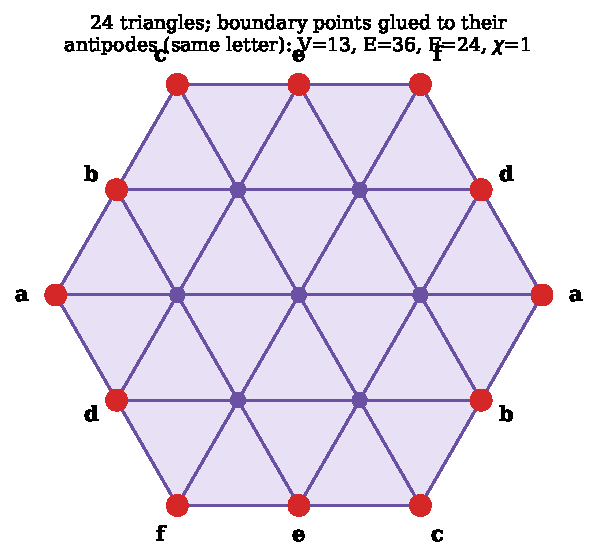
\includegraphics[width=\linewidth]{figures/rp2_hexagon.pdf}
\end{minipage}\hfill
\begin{minipage}{0.5\linewidth}
\caption{The slide's surface, reconstructed: a hexagonal patch of 24 triangles whose boundary vertices with the same
letter (and the boundary edges between them) are identified antipodally. A disc with antipodal boundary points
identified is, by definition, the real projective plane.}\label{fig:rp2}
\end{minipage}
\end{figure}

\begin{proposition}\label{prop:rp2}
The glued hexagon is a triangulation of the real projective plane $\mathbb{RP}^2$. Its Betti numbers are
$(1,0,0)$ over $\QQ$ and $(1,1,1)$ over $\Z_2$, and it admits no coherent orientation.
\end{proposition}
\begin{proof}
A closed disc with antipodal boundary identification is a standard model of $\mathbb{RP}^2$. Independently:
every edge lies in two triangles and every vertex link is a single cycle, so the complex is a closed surface;
the orientation-propagation test fails; and by \cref{thm:classification}, $\chi=1$ with non-orientability gives
$k=1$ cross-cap. The Betti numbers are computed by \code{SimplicialComplex.betti}; the difference between the two
fields reflects $H_1(\mathbb{RP}^2;\Z)=\Z_2$.
\end{proof}

The slide's own reasoning is also correct and worth making explicit: if the surface were orientable, then
$2-2g=1$ would force $g=\tfrac12$, which is impossible. The surface therefore \emph{must} be non-orientable,
which is exactly why the next slide turns to M\"obius strips, Klein bottles and Boy's surface (an immersion of
$\mathbb{RP}^2$ in 3-space).

\section{The pitch-class complex tells a different story}
It is instructive to compare the diagram with the chord complex of Chapter~\ref{ch:topology}, where notes are
vertices. Inside one whole-tone scale (6 notes) there are 6 dominant-seventh shells and 6 major-ninth shells:
\begin{center}\small
\begin{tabular}{@{}lccccl@{}}\toprule
Triangles & $V$ & $E$ & $F$ & $\chi$ & Space\\\midrule
6 dom.-seventh shells $\{r,r{+}4,r{+}10\}$ & 6 & 15 & 6 & $-3$ & orientable, with boundary\\
6 major-ninth shells $\{r,r{+}2,r{+}4\}$ & 6 & 12 & 6 & 0 & cylinder\\
both (12 chords) & 6 & 15 & 12 & 3 & not a surface (see text)\\\bottomrule
\end{tabular}
\end{center}
The combined complex has Betti numbers $(1,0,2)$ and is not a surface at all. Hence the projective plane of the
slide is not the vertex-based chord complex; it is one particular \emph{edge-labelled} gluing, and the choice of
gluing matters. The next section quantifies how much.

\section{Edge-labelled gluings: a census}
\begin{definition}
Given a list of chords, each a triangle whose three edges carry its three notes, an \emph{edge Tonnetz} is obtained
by gluing all edges in pairs, only ever gluing two edges with the same note label, with one of the two possible
orientations for each glued pair.
\end{definition}
Gluing polygons edge-to-edge in pairs always produces a closed surface (possibly disconnected); this is the setting
of the classification theorem. For the 12 shell chords of the whole-tone scale $\{1,3,5,7,9,11\}$ every note
belongs to exactly 6 chords, so each note labels 6 edge slots that must be paired into 3 glued edges: $15$ perfect
matchings times $2^3$ orientations per note, i.e.\ $120^6\approx3\times10^{12}$ gluings. Every one has $F=12$ and
$E=18$, hence $\chi=V-6$, but the number of vertices depends on the gluing.

\begin{figure}[t]\centering
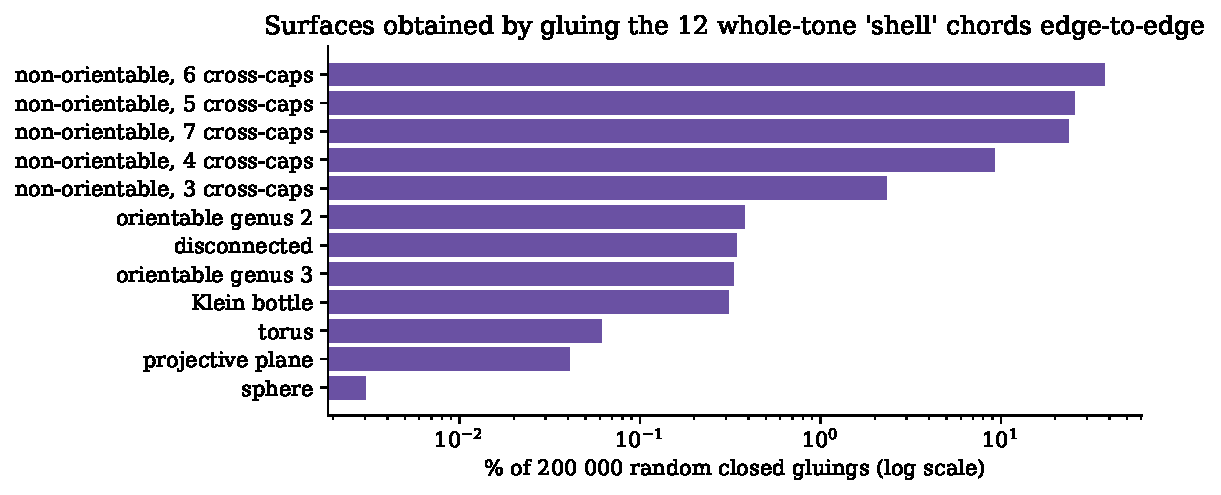
\includegraphics[width=0.86\linewidth]{figures/edge_census.pdf}
\caption{Surfaces obtained from 200\,000 uniformly random closed gluings of the 12 whole-tone shell chords.}
\label{fig:census}
\end{figure}

\Cref{fig:census} shows a Monte-Carlo census of 200\,000 random gluings (\code{sample\_edge\_tonnetze}). The typical
outcome is a non-orientable surface with 5 to 7 cross-caps (together 87\%). Orientable surfaces are rare (0.78\% in
total: genus 2, genus 3, torus, and sphere). The projective plane occurs in only 0.041\% of gluings, and the sphere in 0.003\%.
The surface of the slide is therefore a very special member of a very large family. Two lessons follow.
\begin{enumerate}
\item An edge Tonnetz is not determined by its chord vocabulary alone. A musically motivated gluing rule (for
instance, glue two chords along a note only if they also share a second note, so that adjacent triangles are
parsimoniously related) is needed to make the construction canonical.
\item Finding the gluings with the \emph{largest} Euler characteristic is a combinatorial optimisation problem;
we pose exact enumeration up to symmetry as an open problem in Chapter~\ref{ch:outlook}.
\end{enumerate}

\section{Non-orientable spaces elsewhere in music theory}
Non-orientability is not an exotic accident. The space of unordered two-note chords is a M\"obius band
\citep{callender2008,tymoczko2011}: it is the space of unordered pairs of points on the pitch-class circle, whose
single boundary circle consists of the unisons, and in which the tritones form the central circle of the band. Catanzaro's harmonic strip is a M\"obius band in odd temperaments (Chapter~\ref{ch:topology}), and his
tritone Tonnetze relate to Peck's Klein-bottle Tonnetz \citep{catanzaro2011}. These examples show that the
orientable torus of the classical Tonnetz is a special case, not the norm.

\begin{notebookbox}
\sheet{06\_edge\_tonnetz.ipynb}: rebuild the glued hexagon and verify \cref{prop:rp2}, compute the pitch-class
complexes above, run the census, and search for a spherical gluing.
\end{notebookbox}

\begin{qa}
\Qu{In C7 = C--E--G--B$\flat$, which note is usually omitted in a shell voicing, and why?}
\A{The fifth, G: it adds little to the chord's identity, which is carried by the third (quality) and the seventh
(dominant function).}
\Qu{Verify the counts $V=13$, $E=36$ for the glued hexagon.}
\A{Before gluing: 19 vertices (7 interior, 12 boundary) and 42 edges (30 interior, 12 boundary). Antipodal gluing
halves the boundary: $7+6=13$ vertices and $30+6=36$ edges.}
\Qu{Why must a closed surface with $\chi=1$ be non-orientable?}
\A{Orientable closed surfaces have $\chi=2-2g$, always even.}
\Qu{What are the Betti numbers of $\mathbb{RP}^2$ over $\QQ$ and over $\Z_2$?}
\A{$(1,0,0)$ over $\QQ$ and $(1,1,1)$ over $\Z_2$.}
\Qu{For the 12-chord edge Tonnetz, how many vertices does a spherical gluing have?}
\A{$\chi=V-18+12=2$ gives $V=8$.}
\Qu{Why is the whole-tone pitch-class complex with both chord types not a surface?}
\A{Each whole-tone edge $\{x,x+2\}$ lies in two major-ninth shells and one dominant-seventh shell: three
triangles, whereas a surface allows at most two.}
\end{qa}

\chapter{The Tonnetz meets data}\label{ch:data}
The previous chapters treated the Tonnetz as a mathematical object. This chapter asks how real music moves on it.
We survey public datasets and software, describe a reproducible pipeline, and report a small four-corpus study.

\section{Public datasets}
\Cref{tab:datasets} lists open chord corpora suitable for Tonnetz analysis. They differ in three ways that matter:
\emph{representation} (chord labels such as Harte syntax \citep{harte2005}, Roman numerals, or full scores),
\emph{timing} (aligned to audio or to the score), and \emph{licence}.

\begin{table}[t]\centering\small
\begin{tabular}{@{}p{3.2cm}p{2.5cm}p{3.4cm}p{5.2cm}@{}}\toprule
Dataset & Size & Representation & Access\\\midrule
ChoCo \citep{deberardinis2023} & 18 integrated collections & JAMS; Harte, Roman, lead-sheet & \url{github.com/smashub/choco}, CC BY 4.0 (mostly)\\
Chordonomicon \citep{kantarelis2024} & $>$666\,000 songs & chord symbols + genre, year, sections & \url{github.com/spyroskantarelis/chordonomicon}; Hugging Face\\
ABC: Annotated Beethoven Corpus \citep{neuwirth2018} & 70 quartet movements & DCML harmony labels (TSV) & \url{github.com/DCMLab/ABC}, CC BY-NC-SA 4.0\\
Distant Listening Corpus \citep{hentschel2025} & 1\,326 pieces, 36 composers & DCML standard & \url{github.com/DCMLab/distant_listening_corpus}\\
NYU MARL annotations & 100 RWC-Pop + 195 USPop2002 songs & Harte-syntax \code{.lab} & \url{github.com/tmc323/Chord-Annotations}\\
music21 corpus \citep{cuthbert2010} & $\approx$400 Bach chorale files & full scores (MusicXML) & ships with \code{pip install music21}\\\bottomrule
\end{tabular}
\caption{Open corpora for Tonnetz studies. The last four rows are used in this chapter.}\label{tab:datasets}
\end{table}

\section{A reproducible pipeline}
\paragraph{Parsing.} Harte labels such as \code{A:min7/b3} or \code{C:(1,3,5,b7)} are parsed into pitch-class sets by
\code{harte\_to\_pcs}. DCML annotations list chord tones on the \emph{line of fifths} relative to the local tonic, so
a tone $k$ has pitch class $\text{tonic}+7k \bmod 12$; the local tonic is computed from the global key and the
Roman-numeral local key (\code{dcml\_chord\_pcs}). Bach chorales are ``chordified'' with music21 into vertical
slices.

\paragraph{Reduction to triads.} To place chords on the classical Tonnetz, each chord is reduced to its underlying
major or minor triad when it has one (\code{C:7}$\to$C, \code{A:min7}$\to$Am), following the ``majmin'' reduction
standard in chord-recognition evaluation \citep{raffel2014}. Diminished, augmented and suspended chords are dropped;
consecutive repeats are merged. For the Beethoven corpus we use the first three DCML chord tones (root, third,
fifth), so V$^7$ counts as V. For Bach we keep only slices whose pitch-class content is exactly a consonant triad.

\paragraph{Measurement.} For each pair of consecutive triads we record their distance in $\Gamma$ and their
voice-leading cost. As a \emph{null model} we shuffle the order of chords within each piece (keeping the piece's
chord vocabulary), merge any repeats created, and recompute the mean distance, averaged over 20 shuffles. A corpus
whose progressions are shorter than its own shuffles uses the Tonnetz ``locally'' beyond what its vocabulary alone
implies.

\section{Results}
\begin{table}[t]\centering\footnotesize\setlength{\tabcolsep}{4.5pt}
\begin{tabular}{@{}lrrcccccc@{}}\toprule
Corpus & Pieces & Transitions & Mean $d_\Gamma$ & Shuffled & $P(d{=}1)$ & $P(d{=}2)$ & $P(d{=}4)$ & Mean VL\\\midrule
Bach chorales & 400 & 13\,794 & 2.33 & 2.36 & 0.170 & 0.447 & 0.072 & 3.08\\
Beethoven (ABC) & 70 & 15\,097 & 2.39 & \textbf{2.58} & 0.131 & 0.469 & 0.075 & 3.05\\
RWC Pop & 100 & 11\,737 & 2.62 & \textbf{2.47} & 0.126 & 0.367 & 0.215 & 3.67\\
USPop2002 subset & 194 & 21\,945 & 2.49 & 2.44 & 0.154 & 0.415 & 0.197 & 3.57\\\midrule
Uniform random & -- & -- & 2.78 & -- & 0.130 & 0.261 & 0.217 & --\\\bottomrule
\end{tabular}
\caption{Consecutive-triad distances on the $PLR$ graph ($d_\Gamma$) and voice-leading cost (VL, semitones).
``Shuffled'' is the mean distance after randomly reordering each piece's chords. Produced by
\code{scripts/corpus\_analysis.py}.}\label{tab:corpus}
\end{table}

\begin{figure}[t]\centering
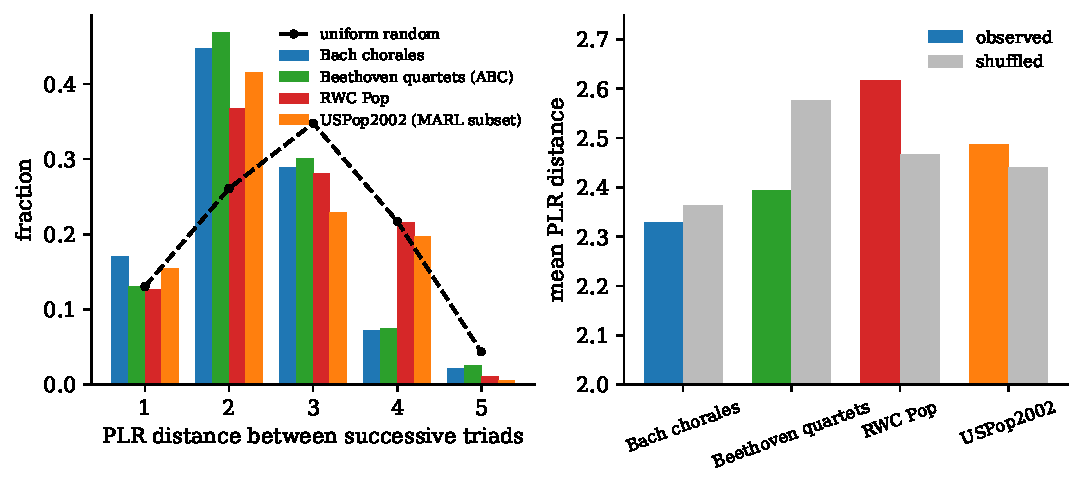
\includegraphics[width=\linewidth]{figures/corpus_plr.pdf}
\caption{Left: distribution of $PLR$ distances between successive triads, with the uniform baseline (dashed).
Right: observed mean distance versus the within-piece shuffle.}\label{fig:corpus}
\end{figure}

\Cref{tab:corpus} and \cref{fig:corpus} support four observations.
\begin{enumerate}
\item \emph{All four corpora are far more local than chance.} Distance 2 dominates everywhere. It is the distance
of motion by fifth (C$\to$G via Em, i.e.\ $L$ then $R$), the backbone of tonal harmony, and of motion by third
(C$\to$Am, C$\to$Em are distance 1).
\item \emph{Classical progressions exploit the Tonnetz beyond their vocabulary.} Beethoven's mean distance (2.39) is
well below that of his own shuffled chords (2.58); Bach's is slightly below (2.33 versus 2.36). The chorale
vocabulary is already so diatonic that shuffling it changes little.
\item \emph{Pop progressions do not.} Both pop corpora are \emph{longer} than their shuffles (RWC 2.62 versus
2.47). Almost the whole difference sits at distance 4, which occurs about three times as often in pop as in the
classical corpora.
\item \emph{Distance 4 in pop is the whole-step move.} Among distance-4 transitions, major-to-major root motion by
a whole step accounts for 77\% in USPop (45\% up, 32\% down) and 67\% in RWC. These are IV$\to$V, $\flat$VII$\to$I and
I$\to\flat$VII, idiomatic in rock \citep{biamonte2010,declercq2011}. In $\Gamma$ they cost four steps; in voice
leading they cost 6 semitones (all three voices move by a tone) against 3 for motion by fifth.
\end{enumerate}
The last point is a caution as much as a finding. The Tonnetz metric encodes a specific theory of closeness
(common tones and semitone voice leading). Pop's parallel whole-step motion is ``far'' under that theory but is not
perceived as a remote relation. Using the Tonnetz as a style descriptor, as in genre classification from Tonnetz
trajectories \citep{karystinaios2020}, measures distance from that theory, not a universal notion of harmonic
distance. Xu, Hall and Rohrmeier reach a related conclusion from pitch distributions: popular music shows higher
tonal focus but classical music more structured traversal of the Tonnetz \citep{xu2026}, building on the Tonal
Diffusion Model \citep{lieck2020}.

\paragraph{Limitations.} The reductions discard information (all seventh chords collapse to triads, and in Bach
non-triadic slices are skipped, which can create artificial jumps). The pop annotations are by trained students and
the classical ones by experts; annotation conventions differ. The corpora are small by modern standards; running
the same script on ChoCo or Chordonomicon would test whether the pattern generalises across genres and decades.

\section{From audio: the tonal centroid}
Harte, Sandler and Gasser \citep{harte2006} map a 12-bin chroma vector $c$ (energy per pitch class) to a point in
$\mathbb R^6$:
\[
\zeta(c)=\frac{1}{\|c\|_1}\sum_{\ell=0}^{11}c_\ell\,\Phi_\ell,\qquad
\Phi_\ell=\bigl(r_1\sin\tfrac{7\pi\ell}{6},\,r_1\cos\tfrac{7\pi\ell}{6},\,r_2\sin\tfrac{3\pi\ell}{2},\,r_2\cos\tfrac{3\pi\ell}{2},\,
r_3\sin\tfrac{2\pi\ell}{3},\,r_3\cos\tfrac{2\pi\ell}{3}\bigr),
\]
with $(r_1,r_2,r_3)=(1,1,\tfrac12)$. The three coordinate pairs place each pitch class on the circle of fifths, a
circle of minor thirds (4 points) and a circle of major thirds (3 points), which are exactly the three directions of
the Tonnetz; wrapping the lattice onto these circles is a continuous version of \cref{thm:torus}. The Euclidean
distance between successive centroids is the \emph{harmonic change detection function} used to locate chord
changes. Our implementation \code{tonal\_centroid} agrees with \code{librosa.feature.tonnetz} \citep{mcfee2015} to
within $3\times10^{-8}$ on synthesised audio. In centroid space the closest pairs of triads are $R$-related, followed
by $P$- and $L$-related pairs (\cref{fig:centroid}).

\begin{figure}[t]\centering
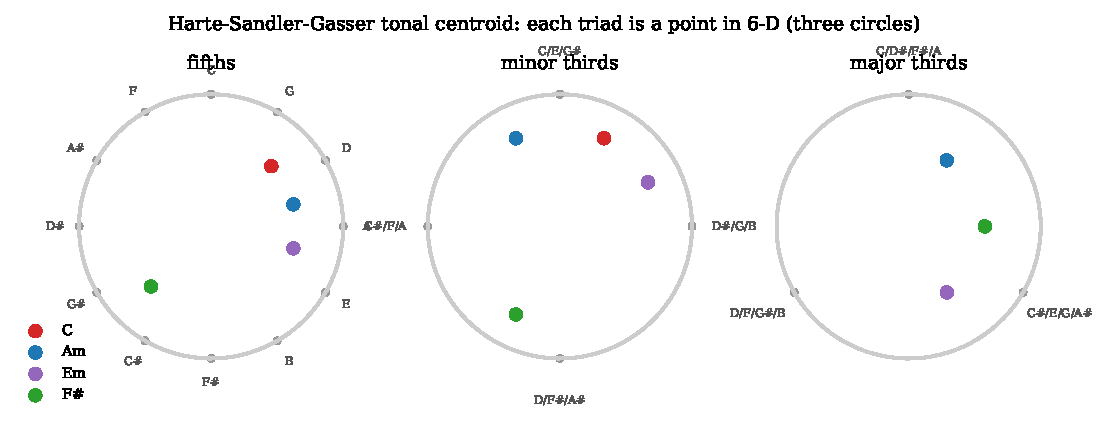
\includegraphics[width=0.92\linewidth]{figures/tonal_centroid.pdf}
\caption{Tonal centroids of four triads on the three circles. C and Am (an $R$ pair) are close on all three.}
\label{fig:centroid}
\end{figure}

\begin{notebookbox}
\sheet{07\_corpus\_analysis.ipynb} reruns \cref{tab:corpus} after \code{bash scripts/fetch\_data.sh};
\sheet{08\_audio\_centroid.ipynb} synthesises a progression, computes chroma, tonal centroid and HCDF, and compares
with librosa.
\end{notebookbox}

\begin{qa}
\Qu{Why reduce C7 to C before measuring Tonnetz distance?}
\A{The classical Tonnetz has only major and minor triads as faces; the reduction keeps the triad that carries the
chord's root and quality and discards the seventh.}
\Qu{What does the within-piece shuffle control for?}
\A{The chord vocabulary. A piece in one key uses nearby triads anyway; comparing with its own shuffles asks
whether the \emph{order} of chords is more local than the vocabulary alone implies.}
\Qu{Why is motion by a perfect fifth at distance 2 in $\Gamma$?}
\A{C$\xrightarrow{L}$Em$\xrightarrow{R}$G: the two triads share one note (G) and are linked through a triad that
shares two notes with each.}
\Qu{Name two reasons why pop corpora show more distance-4 transitions.}
\A{Stepwise root motion between major triads (IV--V, $\flat$VII--I) is idiomatic in rock and pop, and parallel
voice leading is common there; both are ``far'' in a common-tone metric.}
\Qu{How is the tonal centroid related to the Tonnetz?}
\A{It projects pitch classes onto circles of fifths, minor thirds and major thirds, the three lattice directions
of the Tonnetz, and averages over the chord's notes.}
\Qu{Suggest a way to test whether the Beethoven result is specific to Beethoven.}
\A{Run the same pipeline on the Distant Listening Corpus, which uses the same DCML format, grouped by composer and
era, and compare observed-minus-shuffled distances.}
\end{qa}

\chapter{Software ecosystem and open problems}\label{ch:outlook}

\section{Tools}
\begin{table}[h]\centering\small
\begin{tabular}{@{}p{3.0cm}p{7.0cm}p{5.0cm}@{}}\toprule
Tool & What it does & Where\\\midrule
TonnetzViz \citep{cifka2016} & real-time Tonnetz display of MIDI or keyboard input in the browser & \url{github.com/cifkao/tonnetz-viz}\\
HexaChord \citep{bigo2013} & chord complexes, trajectories, compliance measures & Bigo's software page (Java)\\
music21 \citep{cuthbert2010} & score parsing, chordify, Roman numerals, corpus & \code{pip install music21}\\
librosa \citep{mcfee2015} & chroma and tonal-centroid (\code{tonnetz}) features & \code{pip install librosa}\\
mir\_eval \citep{raffel2014} & chord-label parsing and evaluation & \code{pip install mir\_eval}\\
ChoCo tools \citep{deberardinis2023} & JAMS conversion and harmony knowledge graphs & \url{github.com/smashub/choco}\\
\code{tonnetzkit} (this report) & triads, $PLR$, dual graph, Hamiltonian cycles, chord complexes, homology, edge gluings, corpus loaders & companion repository\\\bottomrule
\end{tabular}
\end{table}

\section{Open problems}
The following projects range from student exercises to research questions. Each has a starting point in
\sheet{09\_research\_sandbox.ipynb}.

\paragraph{1. Canonical edge Tonnetze.} Chapter~\ref{ch:nonorient} showed that 12 whole-tone shell chords admit
about $3\times10^{12}$ edge gluings producing surfaces from the sphere to seven cross-caps. Classify them exactly up to
the symmetries of the whole-tone scale, and find a musically motivated gluing rule (for example, requiring adjacent
chords to share two notes) that selects a unique surface. Which rules produce the projective plane of the slide?

\paragraph{2. Hamiltonian cycles for seventh chords.} The graph on the 48 dominant, minor, half-diminished and
major seventh chords, joined when they share three notes, generalises $\Gamma$. How many Hamiltonian cycles does it
have, and how do they fall into symmetry classes? Exhaustive backtracking needs pruning here; compare the seventh-chord
groups of \citep{cannas2017} and the generalized dual of \citep{cannas2018}.

\paragraph{3. Perception.} Test whether listeners prefer Hamiltonian cycles to matched controls (Chapter~\ref{ch:ham}),
and whether ratings track voice-leading cost (28 versus 36 semitones in \cref{tab:ham}).

\paragraph{4. Scaling the corpus study.} Apply the pipeline of Chapter~\ref{ch:data} to ChoCo and Chordonomicon,
stratified by genre and decade. Does the observed-minus-shuffled distance separate styles? Does it change over time?

\paragraph{5. Better metrics.} Combine the Tonnetz metric with voice-leading and functional information, or learn a
metric from data, and compare with Tonnetz-trajectory descriptors \citep{karystinaios2020} and image-like Tonnetz
inputs to neural networks \citep{chuan2018}.

\paragraph{6. Topological fingerprints.} Compute persistent homology of the chord complexes visited by pieces
\citep{bergomi2016}, and relate Betti-number signatures to style.

\paragraph{7. Configurations.} Boland and Hughston interpret the Tonnetz via its Levi graph as a $(12_3)$
configuration and build analogous tone networks for pentatonic and diatonic systems \citep{boland2025,boland2026}.
Which of their networks carry Hamiltonian cycles, and what are their dual surfaces?

\section{Conclusion}
Euler's small lattice of fifths and thirds turns out to be a triangulated torus, a Cayley-like graph of a dihedral
group, and a coordinate system for real music. Its dual graph has exactly 62 Hamiltonian cycles in eight symmetry
classes; its generalizations produce cylinders, spheres, M\"obius bands and, once chords are glued along notes,
projective planes and higher non-orientable surfaces. Placed against data, it separates the common-tone logic of
classical progressions from the whole-step logic of pop. The Tonnetz is best seen not as the one true map of
harmony but as a precise mathematical model whose predictions can be computed, tested and refined, which is what
the accompanying Python sheets are designed to let readers do.

\begin{qa}
\Qu{Why is exhaustive search harder for seventh chords than for triads?}
\A{The graph is larger (48 vertices) and has higher degree, so the number of partial paths grows much faster; pruning
(e.g.\ forcing edges at degree-2 vertices of the remaining graph) or dedicated solvers become necessary.}
\Qu{What would a positive result in open problem 4 look like?}
\A{A stable, significant difference in observed-minus-shuffled Tonnetz distance between genres or eras across
large corpora, robust to the choice of chord reduction.}
\Qu{Give one limitation of the Tonnetz as a model of harmonic distance.}
\A{It ignores function and register and treats stepwise parallel motion between major triads as far, although such
motion is idiomatic and not perceived as remote in pop.}
\Qu{Which chapter's result would you extend first, and why?}
\A{Any answer with a reason is acceptable; for example, Chapter~\ref{ch:nonorient}, because the space of edge gluings
is large, little studied and computationally accessible with the provided code.}
\end{qa}


\appendix
\chapter{Repository guide and reproduction}\label{app:repo}

\section{Layout}
\begin{lstlisting}[language={}]
tonnetz-tutorial/
  tonnetzkit/   core.py (triads, P/L/R)
                graphs.py (dual graph, Hamiltonian cycles)
                topology.py (complexes, homology, orientability)
                edge_tonnetz.py (edge gluings)
                chords.py (parsers, loaders, tonal centroid)
  book/         00_welcome ... 09_research_sandbox.ipynb, _toc.yml
  scripts/      fetch_data.sh, corpus_analysis.py, make_figures.py
  report/       main.tex, ch*.tex, references.bib, figures/
  results/      corpus_stats.json
  tests/        test_tonnetzkit.py (pins every number in the report)
\end{lstlisting}

\section{Reproducing everything}
\begin{lstlisting}[language=bash]
pip install -e ".[dev,audio,corpora]"      # or: pip install -r requirements.txt
pytest -q                                   # 8 tests, about 2 s
bash scripts/fetch_data.sh                  # Beethoven (ABC) + NYU MARL chord labels
python scripts/corpus_analysis.py           # Table 8.2 -> results/corpus_stats.json
python scripts/make_figures.py              # all figures -> report/figures/
jupyter-book build book/                    # the Python sheets as a website
cd report && latexmk -pdf main.tex          # this report
\end{lstlisting}
The GitHub Actions workflow in \code{.github/workflows/ci.yml} runs the tests on every push and publishes the
Jupyter Book to GitHub Pages from the \code{main} branch.

\section{Map from chapters to sheets}
\begin{center}\footnotesize
\begin{tabular}{@{}p{2.8cm}p{4.4cm}p{8.2cm}@{}}\toprule
Chapter & Sheet & Main functions\\\midrule
2 Preliminaries & \code{01\_pitch\_classes} & \code{pc}, \code{transpose}, \code{invert}, \code{trichord\_classes}\\
3 Tonnetz & \code{02\_tonnetz\_torus} & \code{generalized\_tonnetz}, \code{classify\_surface}\\
4 $PLR$ & \code{03\_plr\_dual} & \code{P}, \code{L}, \code{R}, \code{plr\_graph}, \code{apply\_word}\\
5 Hamiltonian & \code{04\_hamiltonian} & \code{hamiltonian\_cycles}, \code{symmetry\_classes}\\
6 Topology & \code{05\_generalized\_tonnetze} & \code{SimplicialComplex.betti}, \code{is\_orientable}\\
7 Non-orientable & \code{06\_edge\_tonnetz} & \code{essential\_notes}, \code{sample\_edge\_tonnetze}\\
8 Data & \code{07\_corpus\_analysis},\newline\code{08\_audio\_centroid} & \code{harte\_to\_triad}, \code{load\_dcml\_corpus}, \code{tonal\_centroid}\\
9 Outlook & \code{09\_research\_sandbox} & --\\\bottomrule
\end{tabular}
\end{center}

\section{Data licences}
The repository contains no third-party data. \code{fetch\_data.sh} downloads the Annotated Beethoven Corpus
(CC BY-NC-SA 4.0; cite \citep{neuwirth2018}) and the NYU MARL chord annotations (cite the repository and the RWC
database \citep{goto2002}); Bach chorales are loaded from the music21 corpus. Users must respect each source's terms.


\chapter*{Acknowledgements}
\addcontentsline{toc}{chapter}{Acknowledgements}
This report grew out of a DREAMS 2025 group project. I thank my co-presenters Saoirse Doran and Kyle Tsang, whose
diagrams (the hand-drawn dual graph and the whole-tone ``edge Tonnetz'') are the starting point of Chapters~4 and~7,
and our advisor James Jones for guidance. I am grateful to the maintainers of the open datasets and software used
here: DCMLab (ABC corpus), NYU MARL (RWC-Pop and USPop chord annotations), the music21, librosa and NetworkX
projects, and O.~C\'ifka for TonnetzViz, whose layout inspired the slide figures.

\bibliographystyle{abbrvnat}
\bibliography{references}
\end{document}
